The lead shield and the active vetos, described above, were included in the simulation of the Tritium-IFIC-2 prototype. The purpose of these simulations was to quantify the reduction of cosmic background detected by the prototype. For this task, the tritium decays was replaced by a cosmic event source, which was simulated using the CRY library. This source of cosmic events consists of a $1 \times 1$ square plane placed on the tritium monitor (at a height of $70~\cm$). The optical properties of the plastic scintillators of the active veto considered are the refractive index, the light attenuation spectrum and energy emission spectrum, the values of which were obtained from their data sheet provided by the manufacturer \cite{ScintillatorVeto}. Two PMTs, model R8520-460 from Hamamatsu, were simulated to read each plastic scintillator, as described in section \ref{subsec:SetUpActiveShield}. The lead shield was simulated with the properties taken from the Geant4 NIST database. The dimensions of the simulated lead shield were $60 \times 60 \times 70~\cm^3$, which are the minimum dimensions needed to fit an active veto and a TRITIUM-IFIC-2 prototype inside it. The length of the simulated lead castle, $60~\cm$, is smaller than the real dimension, $148~\cm$, of the lead shield at Arrocampo. The reason for this is that only one tritium detector module was simulated, so the dimension of the lead shield was reduced to optimize simulation time and computing resources. As for the simulations of the TRITIUM-IFIC-2 prototype, the characteristics of the events generated (energy distribution, position and momentum distribution, etc) were checked to verify the simulation.

Three different simulations were carried out with three different shielding configurations with the aim of quantifying the background rejection due to each part of the background rejection system (pasive shield and active veto). The first simulation consists of a TRITIUM-IFIC-2 prototype and the cosmic ray source. In the second simulation, a lead shield was added and for the third simulation, the cosmic veto was also included. The total counts of cosmic events detected by the TRITIUM-IFIC-2 prototype are shown in Figure \ref{fig:CosmicEventsSuppressionSimulated}, which is divided into three different bins according to the three shielding configurations used. It is found that the cosmic rays detected by the TRITIUM-IFIC-2 prototype are reduced by around a factor 5.5 when a lead shield with $5~\cm$ tick walls is included (the width of the shield currently installed in Arrocampo). This reduction is most probably caused by the suppression of the soft cosmic radiation (energy lower than $200~\MeV$). It has to be taken into account that the natural background of the installation site was not included in this simulation. This radioactive background is also mitigated by the lead shield, so the expected reduction of the radioactive background due to the passive veto would be even better. Around $60\%$ of the cosmic events that penetrate the lead shield and reach the TRITIUM IFIC 2 prototype, which are mostly hard cosmic rays, are detected by the cosmic veto and, therefore, would be mitigated from the background in the detector. In summary, the cosmic events that would be detected by the TRITIUM-IFIC-2 prototype and computed as tritium events are reduced by $92.6\%$ by means of this background rejection system. Furthermore, this reduction is expected to be even larger since, as stated before, the natural background of the site was not included in this simulation.

\begin{figure}[h]
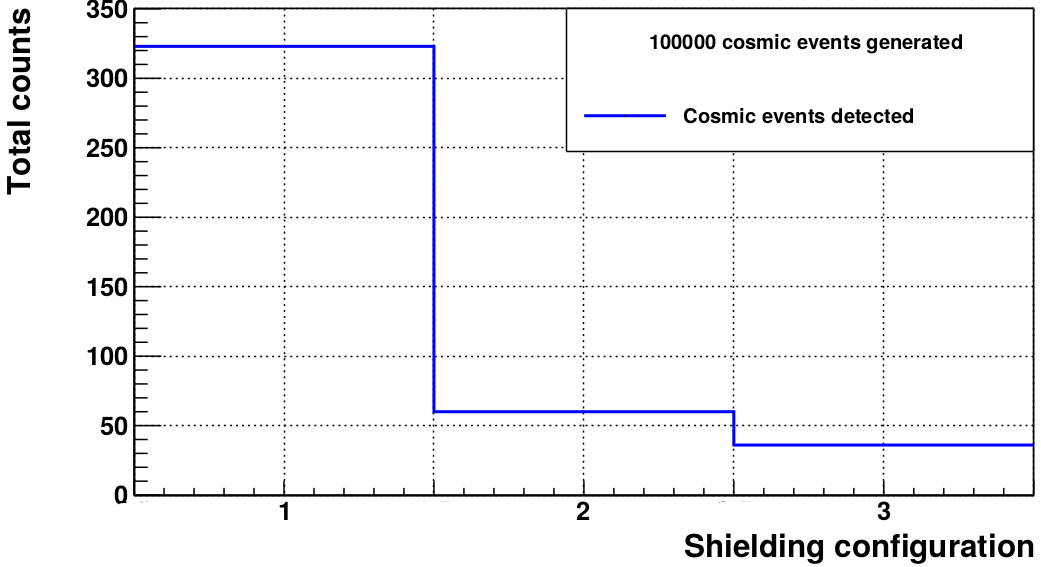
\includegraphics[scale=0.5]{6Simulations/62TRITIUMMonitor/622BackgroundRejectionSystem/Suppression_of_cosmic_events.png}
\centering
\caption{Total cosmic ray events detected by the TRITIUM-IFIC-2 prototype (from a $10^5$ generated cosmic events), which are not candidate events to be suppresed by the background rejection system for three different shielding configuration. The first bin corresponds to a TRITIUM-IFIC-2 prototype without the background rejection system. In the second bin, the passive shield was added to the simulation. In the third bin, the active veto was also included in this simulation.  \label{fig:CosmicEventsSuppressionSimulated}.}
\end{figure}